%!TEX root = ../main.tex

\chapter{Caso studio: comportamento campo fotovoltaico al variare della longitudine}
\label{chp:Caso studio: comportamento campo fotovoltaico al variare della longitudine}
Dopo un'attenta analisi dello strumento(PVGIS) l'obbiettivo di questo capitolo è stato quello di selezionare dieci luoghi a differenti latitudine tenendo fissata la longitudine del polo scientifico dell'università di udine.
\section{La selezione dei luoghi}
La selezione è avvenuta tenendo conto di diversi parametri oltre a quello sopraccitato, ogni regione è stata scelta cercando di attraversare ambienti diversi cercando di distribuire i punti in modo equo sul meridiano partendo da nord per arrivare fino all'equatore.
I parametri con i quali si è effettuata la scelta dei luoghi sono stati i seguenti:
\begin{itemize}
    \item rapporto tra radiazione diffusa e radiazione globale
    \item linea d'orizzonte libera sfruttando lo strumento in figura \ref{fig:orizzonte}
    \item analisi visiva del terreno per selezionare un luogo privo di impedimenti naturali od artificiali
    \item presenza di infrastrutture per il collegamento dell'ipotetico impianto
\end{itemize}
\noindent
Tutti questi parametri sono ovviamente stati calati alla singola regione in cui è stata effettuata l'analisi, in alcune regione desertiche ad esempio il rapporto tra radiazione diffusa e globale è particolarmente basso rispetto a quello che si può trovare ad esempio nelle regioni scandinave.
Per ogni luogo si è cercato di evitare di selezionare un ambiente con caratteristiche peculiari rispetto alla regione di appartenenza, andando ad eliminare luoghi che risulterebbero degli \enquote{outliers} andando a falsare i risultato dello studio.
\paragraph{I luoghi}\mbox{}\\
La scelta è ricaduta su 10 luoghi, ma maggior parte concentrati in Europa in quanto avente un clima vario anche a distanza di pochi chilometri:
\begin{table}[ht]
    \centering
    \begin{tabular}{|lll|}
    \hline
        \textbf{Location} & \textbf{Latitudine} & \textbf{Longitudine} \\ \hline
        Norvegia & 66.280 & 13.216 \\ \hline
        Svezia & 56.707 & 13.217 \\ \hline
        Germania & 52.211 & 13.215 \\ \hline
        Austria & 47.856 & 13.216 \\ \hline
        Friuli Venezia Giulia & 46.079 & 13.213 \\ \hline
        Lazio & 41.670 & 13.218 \\ \hline
        Sicilia & 37.527 & 13.210 \\ \hline
        Libia & 26.579 & 13.216 \\ \hline
        Nigeria & 12.470 & 13.214 \\ \hline
        Gabon & 0.739 & 13.211 \\ \hline
    \end{tabular}
    \label{tab:coordinate}
\end{table}
\begin{figure}[H]
    \centering
    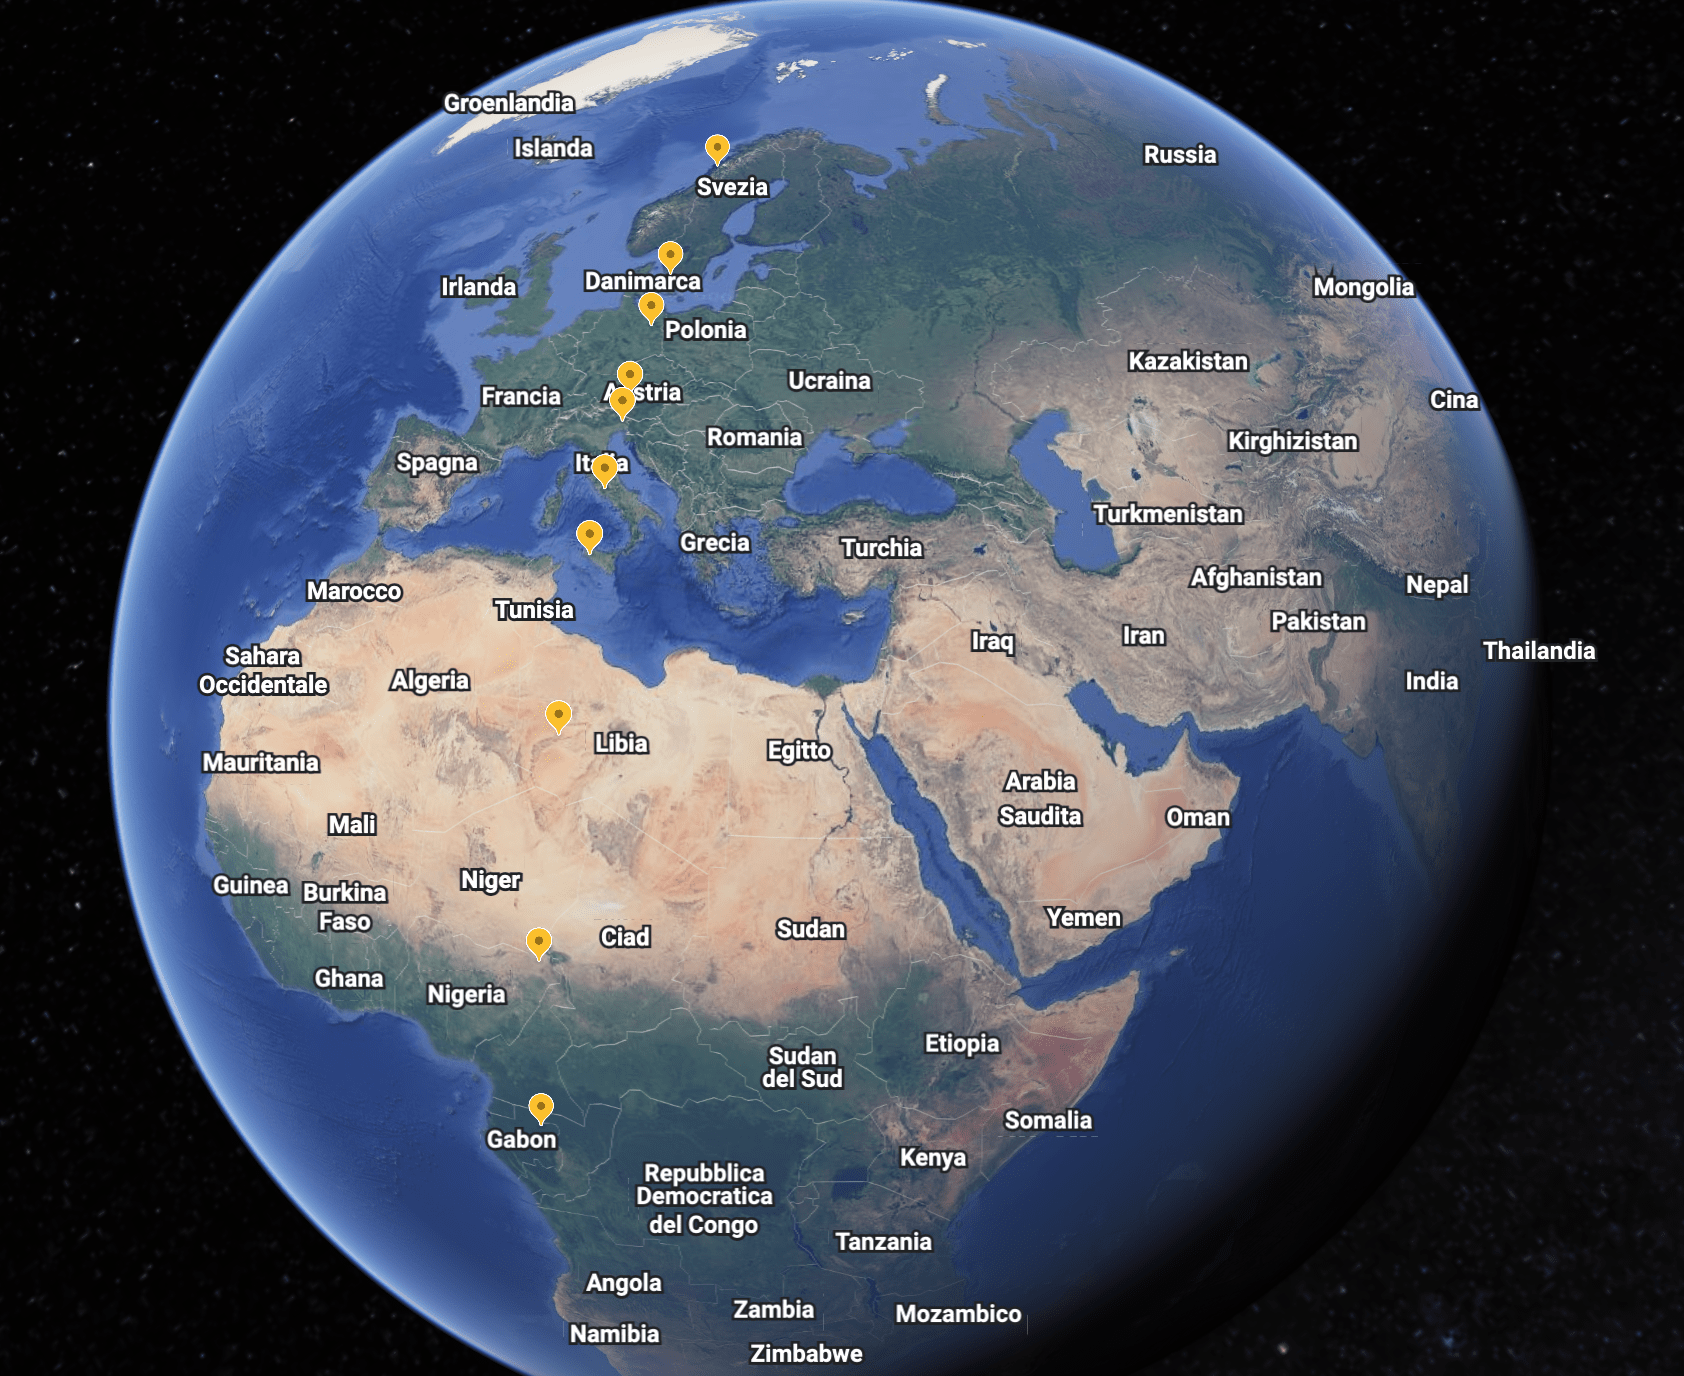
\includegraphics[width=0.9\textwidth]{res/cap 5/map.png}
    \caption{Mappa contenente luoghi scelti}
    \label{img:Mappa luoghi}
\end{figure}\noindent
Come visibile dalla mappa e dalla tabella soprastante i luoghi seguono quasi precisamente la stessa la longitudine e si collocano in 8 stati distinti.\\
Le maggiori difficoltà riscontate nella selezioni dei luoghi sono state sostanzialmente dovute ai seguenti motivi:
\begin{itemize}
    \item Nelle regioni nordiche il meteo varia molto velocemente quindi questo parametro purtroppo non è stato quasi considerato durante la selezione, la longitudine scelta attraversava a nord quasi solamente la zona dei fiordi portando quindi difficoltà nel trovare un'orizzonte libero
    \item Nella zona limitrofa all'arco alpino anche in questo caso la presenza di una catena montuosa ha generato zone di particolare nuvolosità ed anche in questo caso problemi dovuti alla ricerca di un'orizzonte libero
    \item Nella zona desertica invece i problemi sopraccitati non si sono ovviamente riscontrati dando invece origine ad un problema di trovare grossi agglomerati urbani o comunque zone popolate in cui collocare l'impianto
\end{itemize}
\noindent
\section{Simulazione}
In questa sezione tratterò l'analisi numerica dei singoli luoghi in modo da poter analizzare i dati raccolti nella successiva sezione.
La simulazione, come precedentemente anticipato, sarà effettuata su un impianto di \large{$1Kwp$} installato a terra e lasciando scegliere al software sia l'angolo di inclinazione che quello di orientamento, la perdita considerata sarà lasciata impostata al \large{$14\%$} in quanto ritenuto un valore medio di diferimento.\\
Per ogni location sarà quindi eseguita una simulazione simile a quella effettuata nel capitolo precedente in figura \ref{fig:export}.
Saranno inoltre inseriti dati statisti sul rapporto di diffusione(Kd) e sulla temperatura media,estratti dalla scheda in figura \ref{fig:export mensile}, considerando dati mensili tra il 2005 ed il 2020. I dati, come vedremo successivamente, saranno determinanti per valutare l'efficienza dell'installazione.\\
Successivamente saranno inseriti solo i luoghi che abbiano delle caratteristiche peculiari che può essere utile far notare.\\
\newpage
\subsection{Norvegia}
\begin{figure}[H]
    \centering
    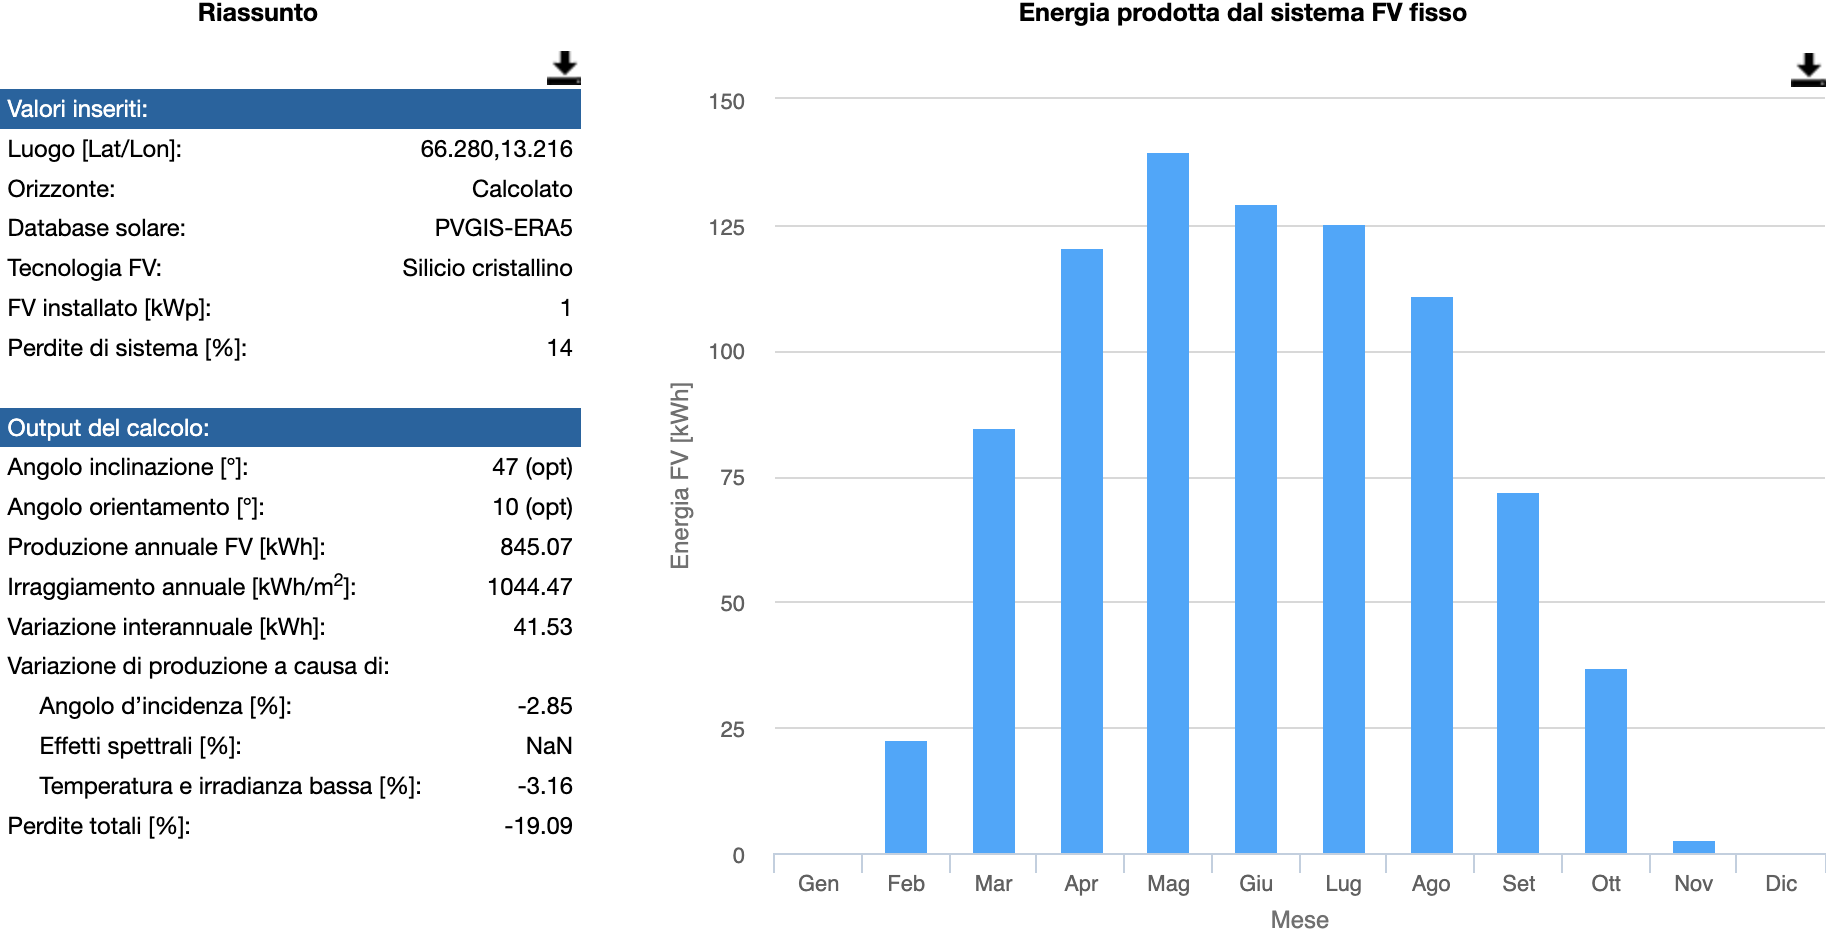
\includegraphics[width=0.7\textwidth]{res/cap 5/impianto norvegia}
\end{figure}\noindent
Come possiamo notare dai dai soprastanti in questo caso i moduli presentano un'angolo di inclinazione piuttosto elevato in quanto risulta l'unico modo per avere un buon rendimento ad latitudini elevate. Si nota come l'angolo di orientamento non sia esattamente zero, ciò è causato da un orizzonte a sud non perfettamente libero, risulta infatti trovato un'orizzonte più pulito a sud-ovest da qui i 10 gradi di orientamento.\\
A primo impatto si nota inoltre come la produzione nei mesi di novembre dicembre e gennaio sia pressocchè nulla, ciò è ovviamente dovuto alla notte polare, in quei mesi infatti il sole non sorgendo non permette ai moduli fotovoltaici di lavorare. Questo fenomeno man mano che ci si dirige verso sud viene sempre più attenuato.
Procediamo ora con un'analisi del Kd e della temperatura media:
\begin{table}[H]
    \centering
    \begin{tabular}{|l|l|l|}
    \hline
         & \textbf{Kd} & \textbf{Temp $[{}^\circ C]$} \\ \hline
        \textbf{Media} & 0,62 & 2,35 \\ \hline
        \textbf{Dev strd} & 0,23 & 7,33 \\ \hline
        \textbf{Mediana} & 0,54 & 1,50 \\ \hline
        \textbf{Massimo} & 1,00 & 18,60 \\ \hline
        \textbf{Minimo}  & 0,28 & -12,00 \\ \hline
    \end{tabular}
\end{table}\noindent
Dall'analisi numerica dei dati storici si nota come il Kd massimo trovato sia 1 ed è dovuto alla mancanza di radiazione diretta, la poca luce presente infatti è dovuta a sola componente diffusa.\\
La temperatura pur essendo il luogo scelto molto a nord risulta piuttosto e ciò può essere dato dalla vicinanza con un fiordo.
\vfill\newpage
\subsection{Friuli Venezia Giulia}
\begin{figure}[H]
    \centering
    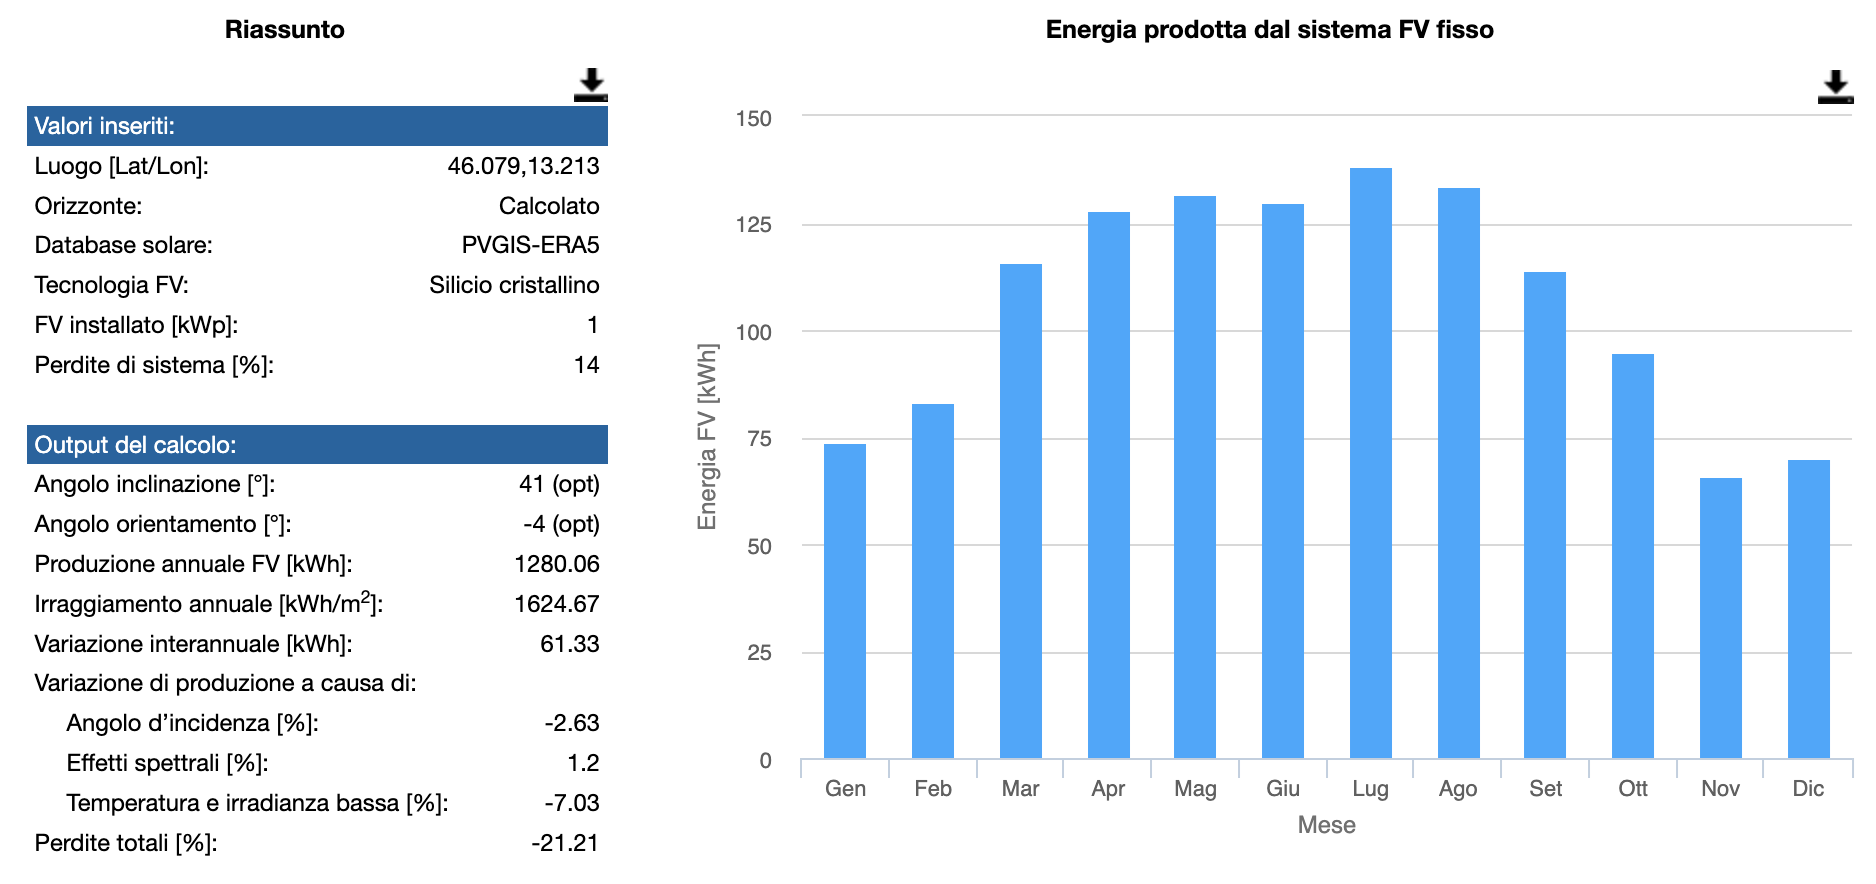
\includegraphics[width=0.7\textwidth]{res/cap 5/impianto udine}
\end{figure}\noindent
Come è possibile notare rispetto alla regione precedente l'angolo di inclinazione dei moduli è sceso con il diminuire della latitudine. La perdita relativa a temperatura e bassa irradianza risulta aumentata infatti come si può vedere dalla tabella sottostante la temperatura media è aumentata di ben 10 gradi rispetto all'estremo nord.\\
Il fenomeno che della notte polare è ovviamente del tutto sparito, ma permane una minor produttività dovuta sia al minor numero di ore di luce che all'arco che il sole compie all'orizzonte non garantendo un'angolo ottimale.\\
Aumentare l'angolo di inclinazione porterebbe infatti giovamento alle prestazioni nei mesi invernali peggiorando però la resa in quelli estivi, nel complesso la produzione annua sarebbe quindi minore.
\begin{table}[H]
    \centering
    \begin{tabular}{|l|l|l|}
    \hline	
          & \textbf{Kd} & \textbf{Temp $[{}^\circ C]$} \\ \hline
        \textbf{Media} & 0,38 & 12,66 \\ \hline
        \textbf{Dev strd} & 0,07 & 7,18 \\ \hline
        \textbf{Mediana} & 0,38 & 12,50 \\ \hline
        \textbf{Massimo} & 0,60 & 25,90 \\ \hline
        \textbf{Minimo} & 0,25 & 0,20 \\ \hline
    \end{tabular}
\end{table}
Il coefficiente diffusione è calato a causa della presenza di un clima più mite ed una minor nuvolosità, i fenomeni che nel nord Italia portano questo parametro a non essere comunque ottimale sono l'elevata presenza di particelle in sospensione nell'ora che portano a fenomeni di diffusione.
\vfill
\newpage
\subsection{Libia}
\begin{figure}[H]
    \centering
    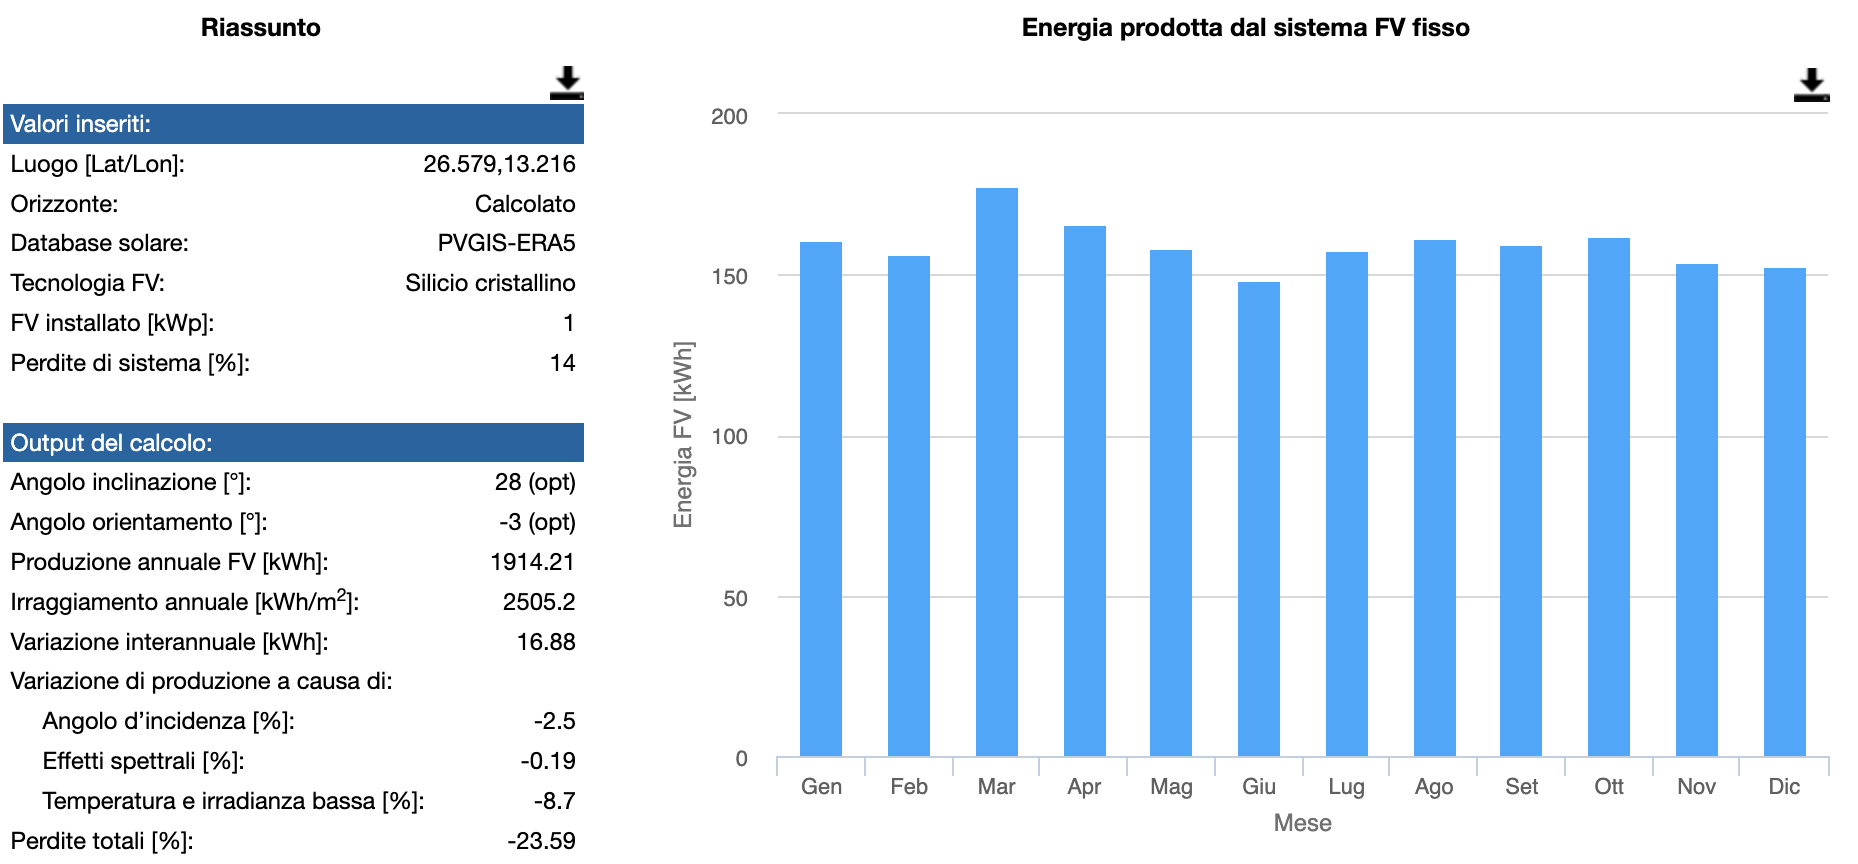
\includegraphics[width=0.7\textwidth]{res/cap 5/impianto libia}
\end{figure}\noindent
L'avvicinamento all'equatore è subito visibili dalla netta diminuzione dell'angolo di inclinazione, non vi è praticamente più una differenza sostanziale tra i vari periodi dell'anno e ciò è ovviamente dovuto ad una minor differenziazione delle stagioni.\\
La produzione risulta ridotta a causa della temperatura che è ovviamente maggiore rispetto alle regioni viste in precedenza e ciò è dovuto alla presenza di un clima sostanzialmente desertico.
\begin{table}[H]
    \centering
    \begin{tabular}{|l|l|l|}
    \hline
          & \textbf{Kd} & \textbf{Temp $[{}^\circ C]$} \\ \hline
        \textbf{Media} & 0,24 & 22,99 \\ \hline
        \textbf{Dev strd} & 0,03 & 7,78 \\ \hline
        \textbf{Mediana} & 0,24 & 22,99 \\ \hline
        \textbf{Massimo} & 0,34 & 33,40 \\ \hline
        \textbf{Minimo} & 0,20 & 8,90 \\ \hline
    \end{tabular}
\end{table}
Il coefficiente di diffusione in questo caso è particolarmente basso e costante, anche qui grazie alla presenza di un clima desertico, la temperatura media e massima per lo stesso motivo si alza notevolmente.
\vfill\newpage
\subsection{Gabon}
\begin{figure}[H]
    \centering
    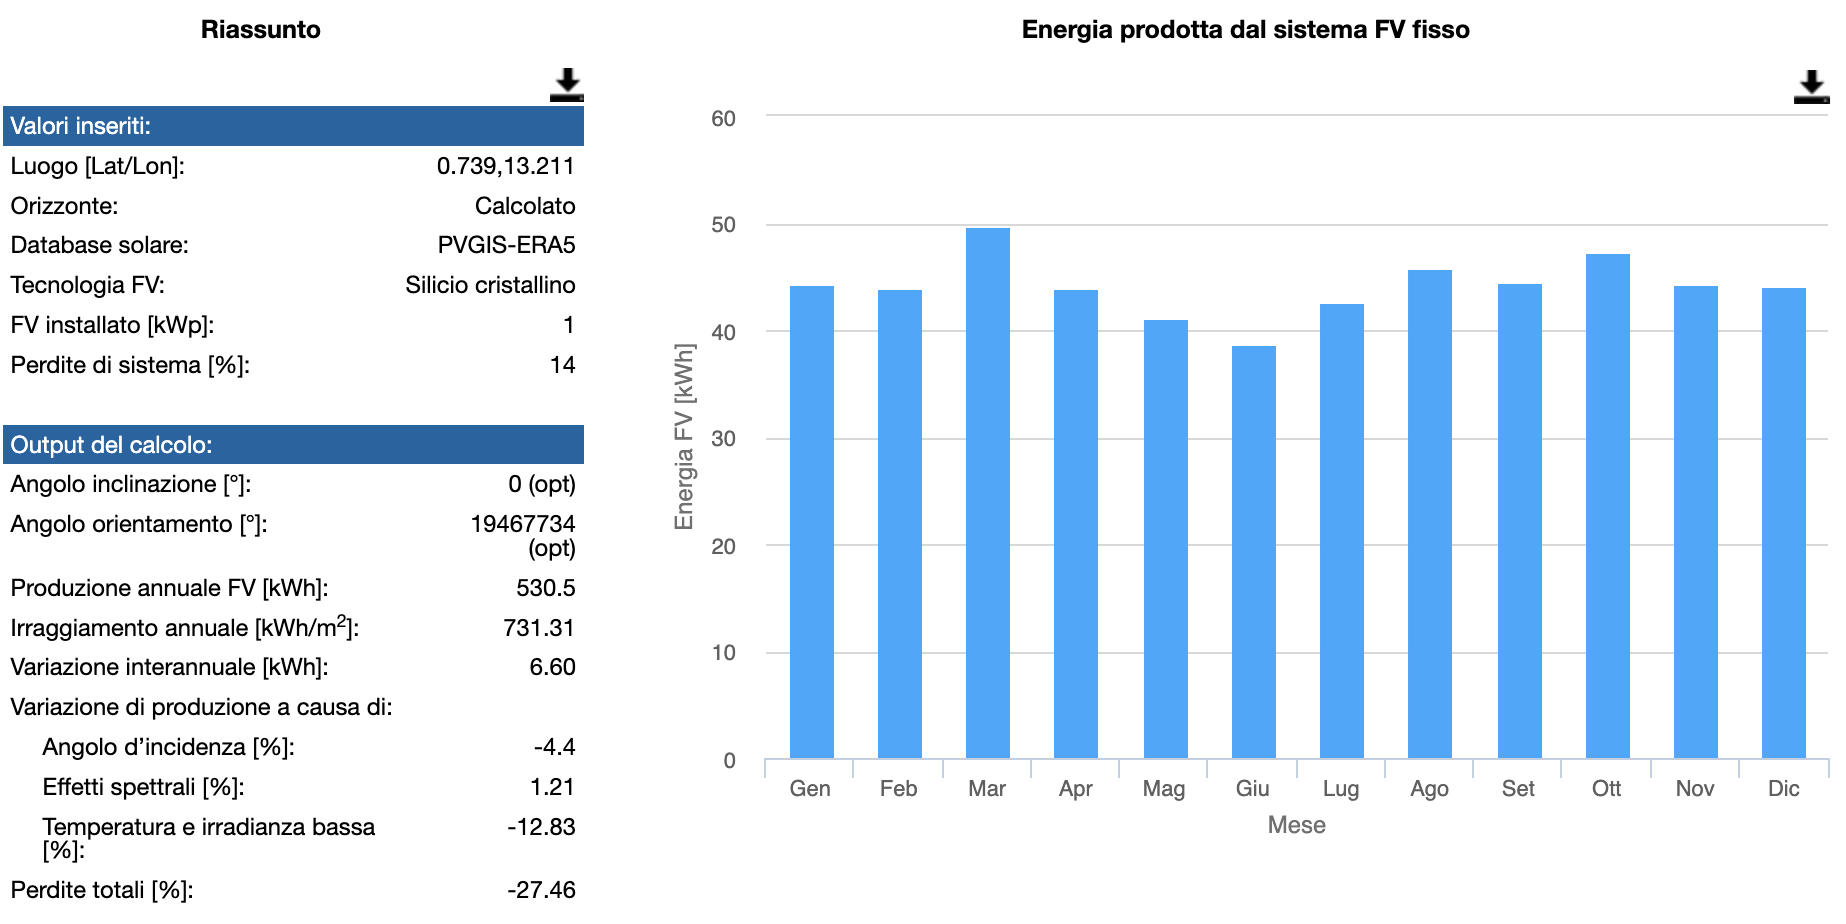
\includegraphics[width=0.7\textwidth]{res/cap 5/impianto gabon}
\end{figure}\noindent
Osservano i dati riguardanti il posizionamento si osserva che l'inclinazione in questo caso è di 0 gradi essendo la componente diretta proveniente già da una direzione perpendicolare. Per quanto riguarda l'orientazione viene erroneamente calcolata in quando per un pannello disposto con un angolo di 0 gradi sul terreno non può essere espresso .\\
In questa regione si nota un fenomeno particolare, ci si aspetterebbe infatti che la zona equatoriale sia quella che riceve una radiazione solare più intensa tuttavia a causa di una non uniforme della radiazione ciò non è del tutto vero.\\
Un altro fenomeno che fa si che l'anello equatoriale scarsamente irradiata è la presenza quasi costante di nuvole e quindi una scarsa componente diretta a favore di una componente diffusa e quindi meno efficace.\\
In un ambiente con le caratteristiche appena viste potrebbe essere interessante utilizzare dei moduli fotovoltaici che presentino una struttura cristallina non orientata la quale garantirebbe una maggior efficienza in caso di componente diffusa altamente presente.
\begin{table}[H]
    \centering
    \begin{tabular}{|l|l|l|}
    \hline	
          & \textbf{Kd} & \textbf{Temp $[{}^\circ C]$} \\ \hline
        \textbf{Media} & 0,45 & 24,44 \\ \hline
        \textbf{Dev strd} & 0,04 & 0,56 \\ \hline
        \textbf{Mediana} & 0,45 & 24,44 \\ \hline
        \textbf{Massimo} & 0,55 & 26,40 \\ \hline
        \textbf{Minimo} & 0,34 & 23,30 \\ \hline
    \end{tabular}
\end{table}
La presenta di un clima particolare è chiaramente evidente osservano i valori statistici ottenuti. Il valore minimo di Kd infatti risulta il maggiore trovato in tutte le regioni precedenti e questo è indice di un clima non ottimale, si riscontra in oltre una media elevata ed una bassa variabilità il che è indice di alta diffusione che permane nel tempo.\\
La temperatura,anche a causa della nuvolosità, risulta più alta ma con massimi più bassi ed una deviazione standard molto più bassa di tutte le regioni desertiche viste in precedenza.Queste caratteristiche sono molto indicative della situazione climatica della regione\\
\section{Analisi e conclusione}
Terminata la descrizione delle singole location è possibile confermare le aspettative iniziali:
\begin{itemize}
    \item Andando verso la zona equatoriale i moduli fotovoltaici avrebbero mantenuto l'orientamento il più possibile a sud e l'inclinazione sarebbe diminuita progressivamente
    \item La presenza di climi caldi ha favorito la riduzione del Kd garantendo quindi un maggior presenza di componente diretta rispetto a quella diffusa
    \item L'aumento della temperatura ha peggiorato tendenzialmente la resa del moduli fotovoltaici ma tale peggioramento è stato irrilevante in quanto l'aumento delle ore di sole ha mitigato notevolmente il problema
\end{itemize}
A differenza delle aspettative iniziali la zona equatoriale non si è rivelata la migliore in cui installare un campo fotovoltaico a causa del fenomeni citati in precedenza.
Compresa l'importanza fondamentale di avere un modulo correttamente orientato ho provveduto a studiare l'angolo ottimale cercando una correlazione con la latitudine e come mi aspettavo ho ottenuto il seguente risultato:
\begin{figure}[H]
    \centering
    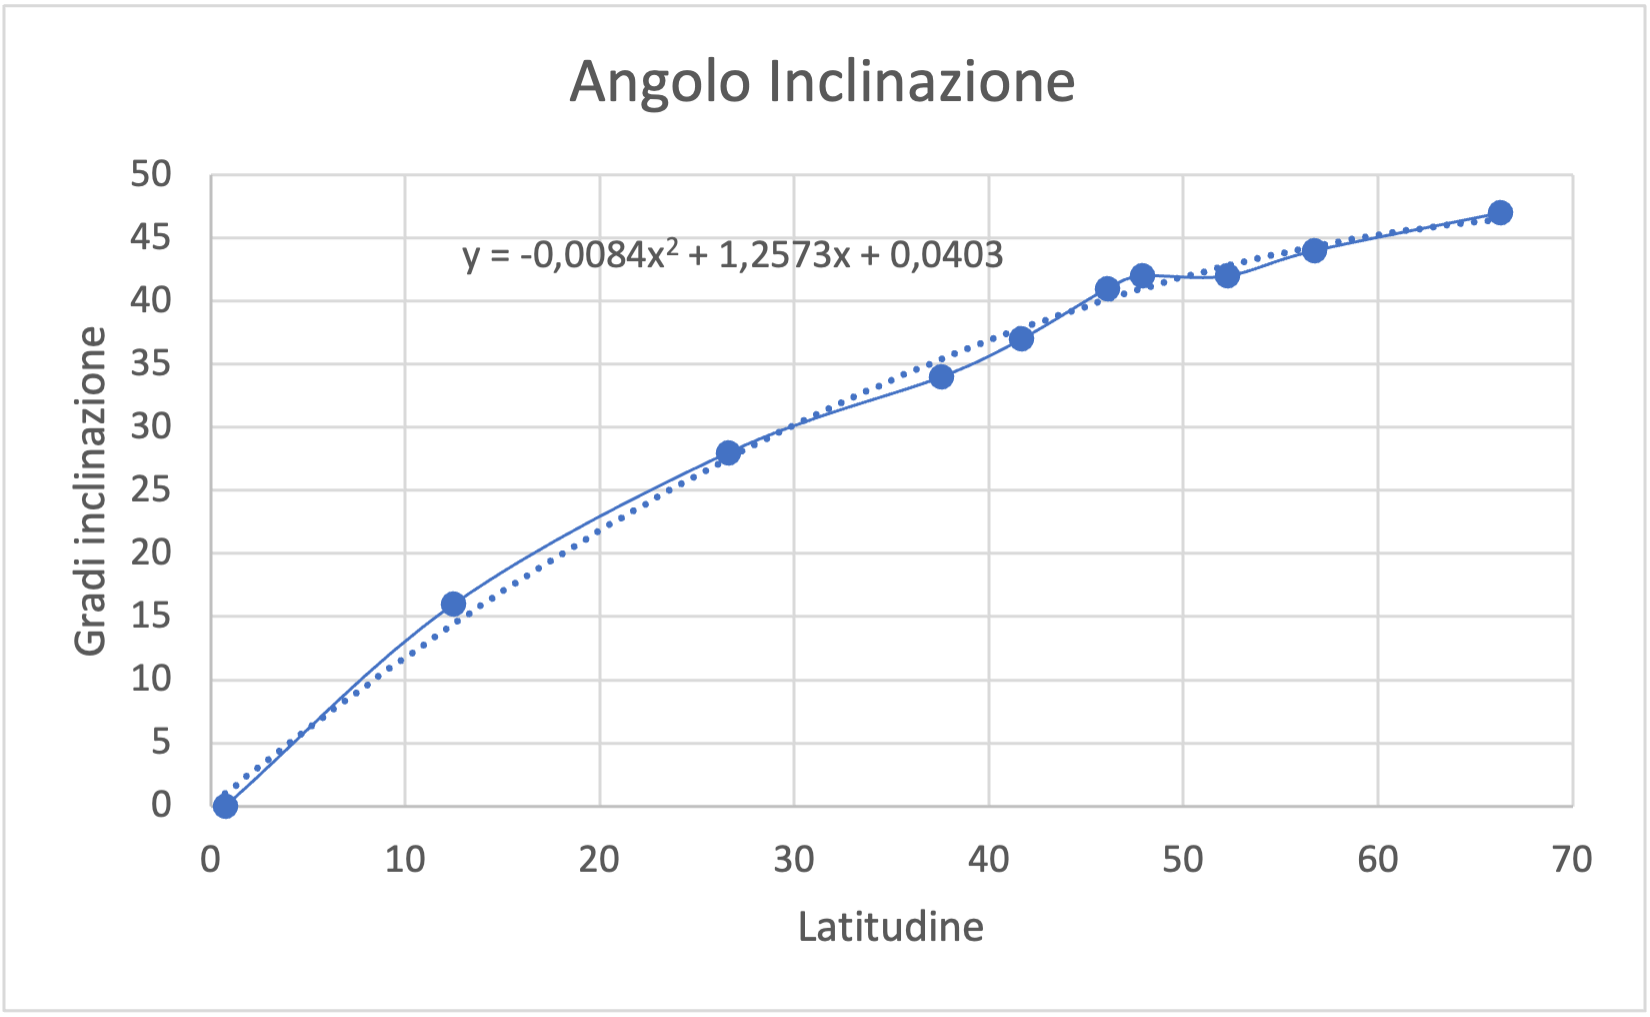
\includegraphics[width=0.8\textwidth]{res/cap 5/regressione lineare}
    \caption{Regressione lineare utilizzando i dati dei luoghi campione}
\end{figure}\noindent
A primo impatto era subito chiaro che vi fosse una funziona di secondo grado che potesse, a partire dalla latitudine, generare l'angolo di inclinazione ottimale. Ho provveduto quindi ad inserire la funzione di regressione lineare ed a graficarla ottenendo la seguente formula:
\begin{center}
    \large{$Angolo\space di\space inclinazione = -0,0084 \cdot (lat)^2 + 1,2573\cdot lat + 0,0403$}
\end{center}
\noindent
Ho provveduto quindi a testare sempre attraverso il tool PVGIS la formula sopra indicato ottenendo un quasi ottimale funzionamento in tutto l'emisfero boreale ad esclusione dei punti più limitrofi al polo nord ma di scarso interesse applicativo in quanto scarsamente popolati e, come visto nel capitolo, non idonei ad ospitare campi fotovoltaici.\\
Per ottenere allo stesso modo un modello capace di restituire l'inclinazione ideale per l'emisfero australe sarebbe sufficiente raccogliere una serie di dati e ripetere la regressione lineare con il nuovo dataset scelto.